\chapter{Language model alignment and applications}


\section{Model alignment}

\begin{remark}
    Off-the-shelf pre-trained models tend to only be good at word completion. They are most likely unable to understand instructions and might generate harmful content.
\end{remark}


\subsection{Instruction tuning}

\begin{description}
    \item[Instruction tuning] \marginnote{Instruction tuning}
        Fine-tune a model on a dataset containing various tasks expressed in natural language in the form $(\text{description}, \text{examples}, \text{solution})$, all possibly formatted using multiple templates.

        \begin{figure}[H]
            \centering
            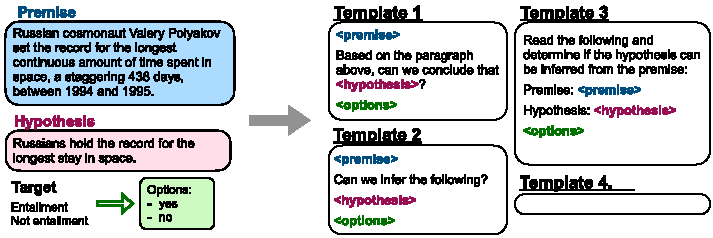
\includegraphics[width=0.7\linewidth]{./img/_instruction_tuning.pdf}
            \caption{Example of templates for entailment detection}
        \end{figure}

        \begin{remark}
            If done correctly, after performing instruction tuning on a model, it should be able to also solve tasks that were not present in the tuning dataset.
        \end{remark}

        \begin{figure}[H]
            \centering
            \begin{subfigure}[c]{0.34\linewidth}
                \centering
                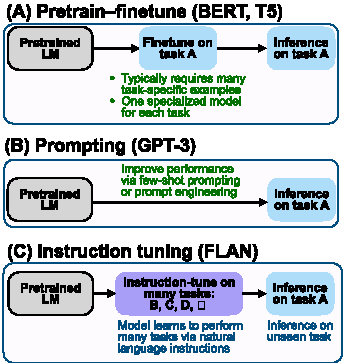
\includegraphics[width=\linewidth]{./img/_tuning_comparison1.pdf}
            \end{subfigure}
            \hfill
            \begin{subfigure}[c]{0.6\linewidth}
                \centering
                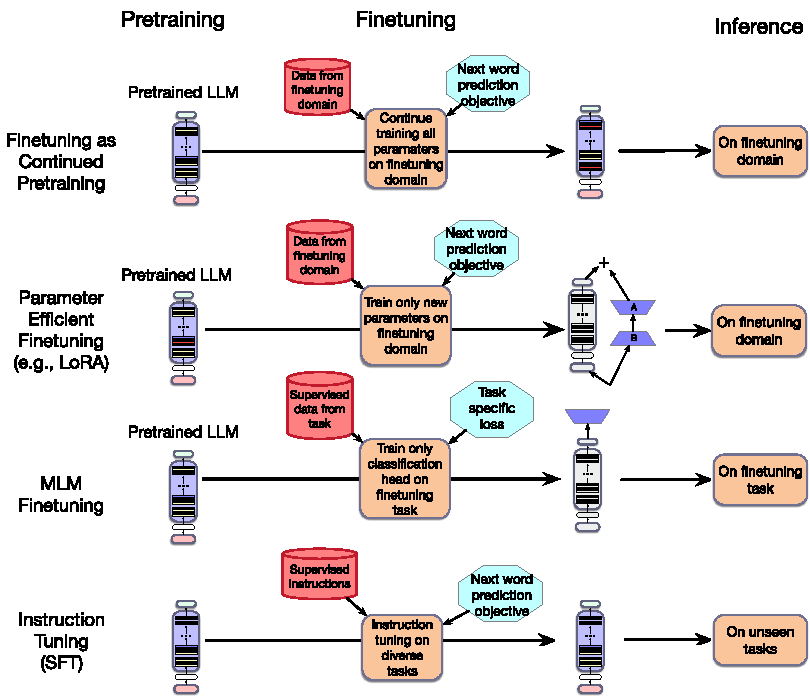
\includegraphics[width=\linewidth]{./img/_tuning_comparison2.pdf}
            \end{subfigure}
            \caption{Comparison of tuning approaches}
        \end{figure}
\end{description}


\subsection{Preference alignment}

\begin{description}
    \item[Preference alignment] \marginnote{Preference alignment}
        Align the output of a model with human values.

    \item[Reinforcement learning with human feedback (RLHF)] \marginnote{Reinforcement learning with human feedback (RLHF)}
        Align a language model using a policy-gradient reinforcement learning algorithm. The problem can be formulated as follows:
        \begin{itemize}
            \item The policy to learn represents the aligned model (i.e., $\texttt{prompt} \mapsto \texttt{answer}$ model),
            \item Prompts are the states,
            \item Answers are the actions.
        \end{itemize}
        RLHF works as follows:
        \begin{enumerate}
            \item Start from a pre-trained language model that already works well.

            \item Train a reward model $r_\theta$ from a human-annotated dataset that maps text sequences into rewards. The architecture is usually based on transformers.

            \item Fine-tune the language model (i.e., train the policy) using an RL algorithm (e.g., PPO) and the learned reward model. 

            Given a prompt $x$ and an answer $y$, the reward $r$ used for the RL update is computed as:
            \[ r = r_\theta(y \mid x) - \lambda_\text{KL} D_\text{KL}(\pi_{\text{PPO}}(y \mid x) \Vert \pi_{\text{base}}(y \mid x)) \]
            where:
            \begin{itemize}
                \item $r_\theta(y \mid x)$ is the reward provided by the reward model.
                \item $- \lambda_\text{KL} D_\text{KL}(\pi_{\text{PPO}}(y \mid x) \Vert \pi_{\text{base}}(y \mid x))$ is a penalty based on the Kullback-Leibler divergence to prevent the aligned model $\pi_\text{PPO}$ from moving too away from the original model $\pi_\text{base}$ (i.e., prevent the loss of language capabilities).
            \end{itemize}
        \end{enumerate}

        \begin{figure}[H]
            \centering
            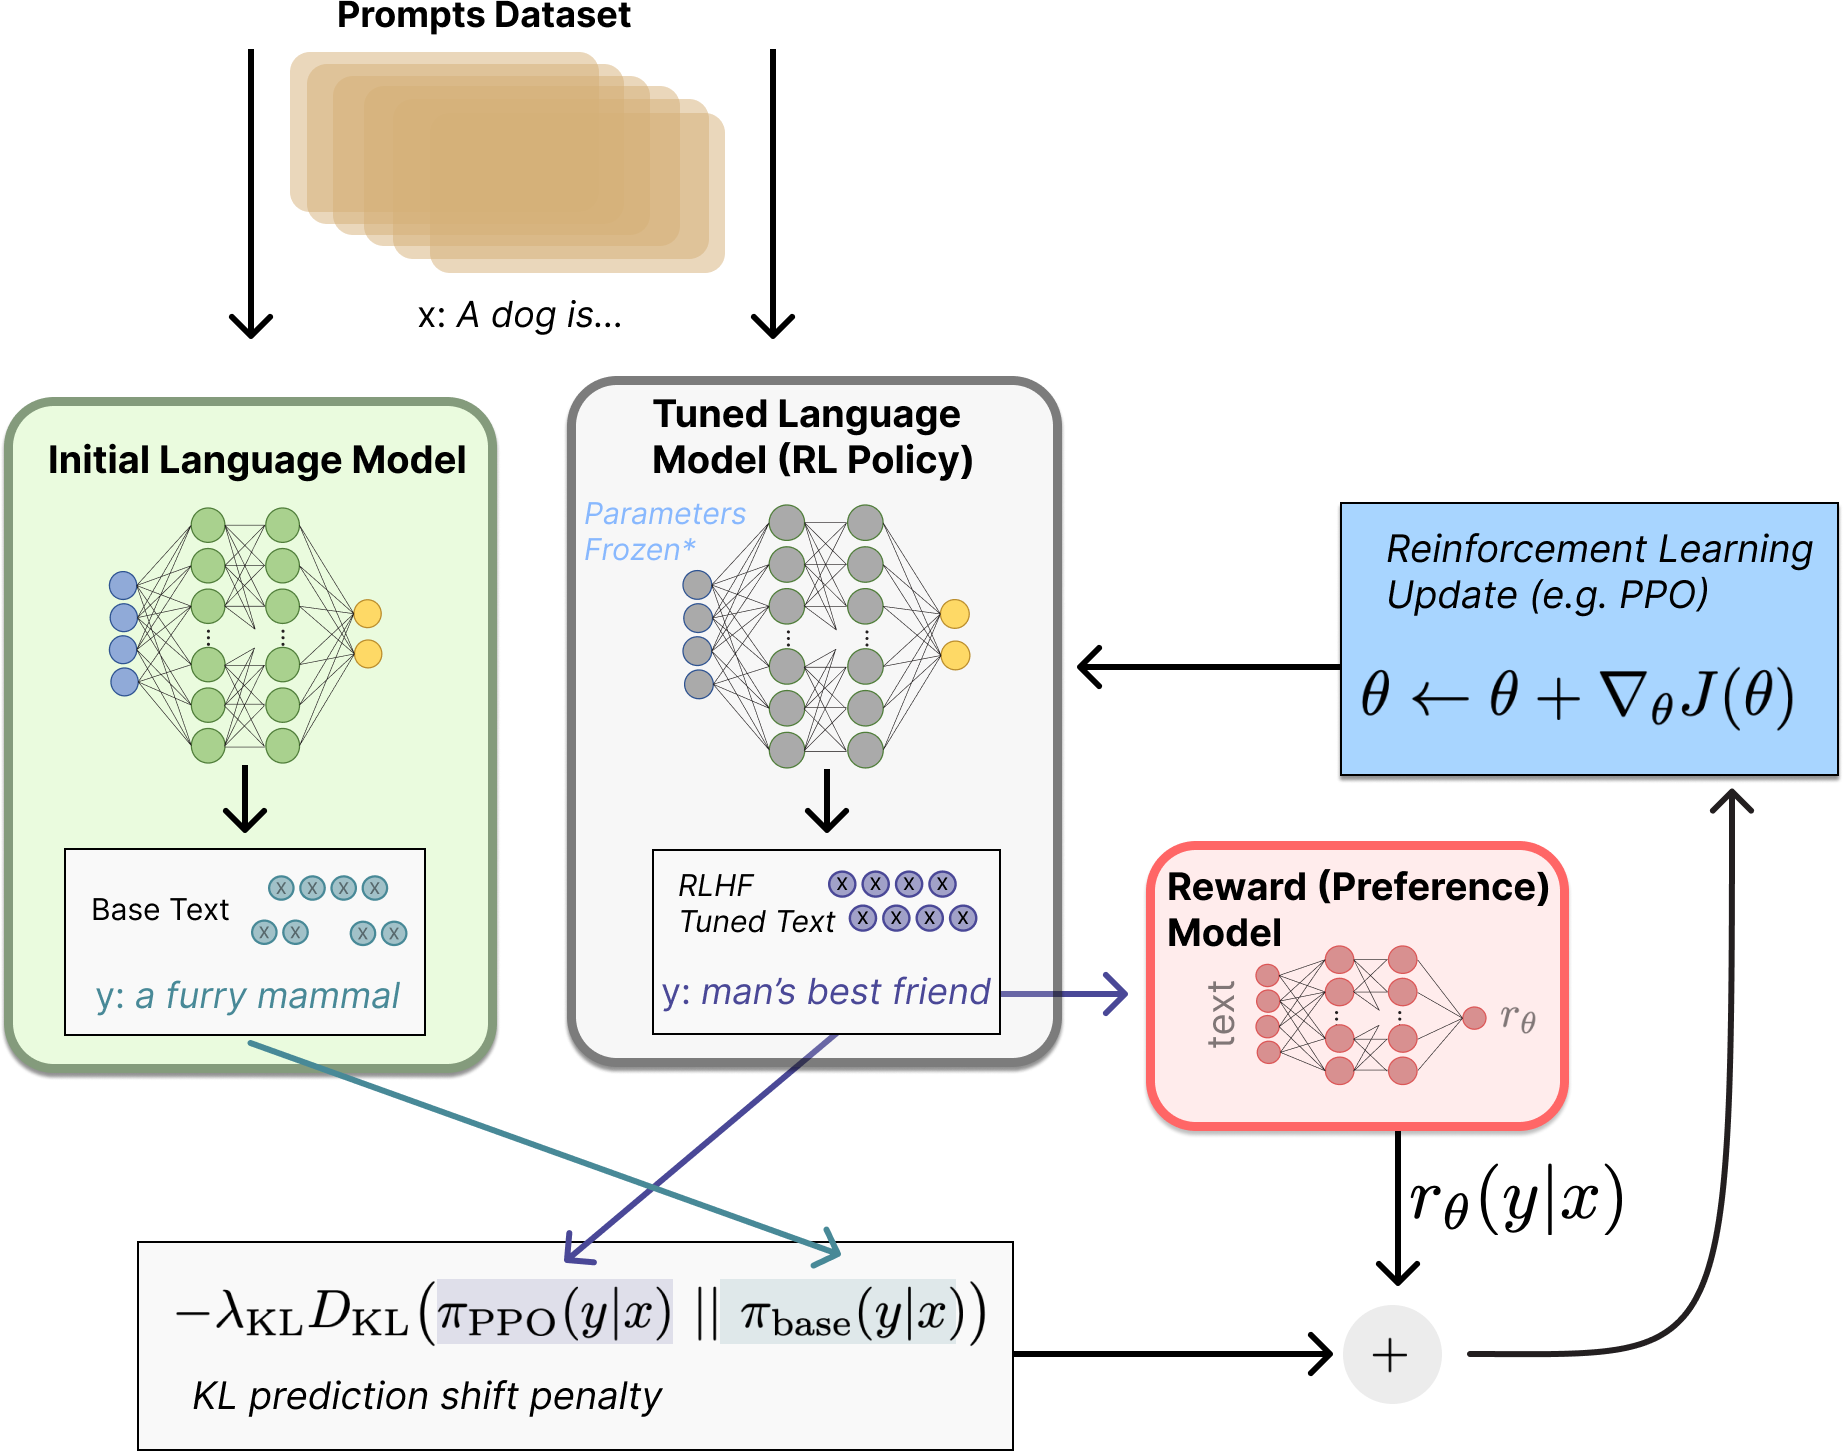
\includegraphics[width=0.6\linewidth]{./img/rlhf.png}
        \end{figure}
\end{description}